% Kirbie Dramdahl Honors Capstone Paper 2015

\documentclass[12pt]{article}

\setlength{\oddsidemargin}{0in}
\setlength{\evensidemargin}{0in}
\setlength{\topmargin}{0in}
\setlength{\headheight}{0in}
\setlength{\headsep}{0in}
\setlength{\textwidth}{6in}
\setlength{\textheight}{9in}
\setlength{\parindent}{0in} 

\usepackage{parskip}
\usepackage{times} %For typeface
\usepackage{graphicx}
\usepackage{algorithm}
\usepackage{algorithm,algorithmic}
\usepackage[justification=centering]{caption}[2007/12/23]
\usepackage{url}
\sloppy

\usepackage{float}
\newfloat{Query}{tbp}{lop}

\newcommand{\inset}[1]{$\in \{ {#1} \}$}

\newcommand{\citep}[1]{\cite{#1}}
\newcommand{\PPLR}[1]{$\eta_M$}
\newcommand{\LLR}[1]{$\eta_L$}

\DeclareGraphicsRule{.tif}{png}{.png}{`convert #1 `dirname #1`/`basename #1 .tif`.png}

\title{Story of Rats:\\
       The Co-Evolution of Rats and Humans}

\author{
 		M. Kirbie Dramdahl\\
        University of Minnesota, Morris\\
        Morris, MN 56267\\
        dramd002@morris.umn.edu\\
}
\date{} 

\begin{document}
\pagestyle{plain}

\maketitle

\begin{abstract}

Humans are currently the most successful species on the planet. We have permeated the globe as a result of our skill at adapting to our environment. But for as long as there have been humans, there have also been rats. And where we have gone, they have followed, with nearly equal success. It is inevitable, therefore, that the lives and histories of rats and humans have become intertwined in complex ways.

Throughout our mutual histories, humans and rats have interacted and affected one another in complex ways. Rats have latched onto humans as providers of food and shelter - whether intentionally or not - while humans have in turn viewed rats as a food source. Rats spread the disease which caused the deaths of millions of humans during the years of the Black Death, while today humans sacrifice the minds and bodies of millions of rats in order to understand their own. Rats are treated as filthy vermin in some contexts, and cherished pets in others. And despite sharing many physical and psychological characteristics with humans, rats are often feared and demonized in human culture.

The purpose of this project is to document and examine the relationship between rats and humans, and how this relationship has affected both species.

\pagebreak

\end{abstract}

\section{Introduction} \label{Introduction}

There are two animals which have found success in nearly every corner of the planet. The first is the human. Approximately 200,000 years ago, the species \textit{Homo sapiens} rose out of Africa and, over time, spread throughout the globe. But where humans went, the second animal, which had already lived for some 1.8 million years, followed. This is the rat. This project addresses the various dynamics of the complex relationship that inevitably developed between rats and humans.

I was interested in taking on this project for two reasons. The first, more specific reason is that my experience with rats is at odds with popular perception. Rats are viewed in most cultures as, at best, pests and, at worst, filthy sources of disease. In my experience, however, having kept pet rats for several years, I have found them to be charming, intelligent, loving creatures. I wanted to undertake this project as a way of connecting and reconciling these two opposite viewpoints, in order to understand the complexities of the relationship between rats and humans.

The second, more general reason is to provide a case study for animal-human relationships in general. The rat is an interesting example because humans have such close, universal contact with rats, and because human attitudes toward rats are so complex. My hope is that in addressing the human perception of rats, light will be shed on the human perception of other species.

This project is divided into several sections. Because the terms ``rat'' and ``human'' may have multiple interpretations, Section~\ref{Definitions} defines these terms as they will be used throughout this project. Section~\ref{Biology} discusses the biological connections between rats and humans, including taxonomy and co-evolutionary patterns. Section~\ref{History} provides an overview of the historical relationships between rats and humans, and Section~\ref{Connections} describes modern developments in this relationship, including the appearance of rats in laboratory research, as companion animals, and in service roles. Any overall conclusions reached over the course of this project are addressed in Section~\ref{Conclusions}.

\section{Definitions} \label{Definitions}

The first issue that must be addressed in discussing the relationships between and co-evolution of rats and humans is to define the subjects in question. Therefore, the first task is to define the terms ``rat'' and ``human.'' The latter term - ``human'' - is simple enough to define. All humans belong to the species \textit{Homo sapiens}, subspecies \textit{Homo sapiens sapiens}, the only surviving species of the genus \textit{Homo}. Regardless of environment, language, religion, ethnicity, race, sex, gender, or any other potentially divisive factor, all members of the species \textit{Homo sapiens} are human.

Defining the former term, however - ``rat'' - requires a bit more consideration. By biological definition, ``true rats'' belong to the genus \textit{Rattus}. While there is a number of extant species belonging to this genus (51 species~\cite{Hanson2012}, 56 species~\cite{EncyclopediaBritannica2014}, and 64 species~\cite{RatWikipedia2014} were a handful of the various counts encountered), this project will predominately focus on two species - \textit{Rattus norvegicus}, the brown rat, and \textit{Rattus rattus}, the black rat. However, this project also mentions a third species, \textit{Cricetomys gambianus}, the giant pouched rat, which is not, in fact, a true rat (Figure~\ref{RatVariationsFigure}). This is because the term ``rat,'' as used in common English language and in reference to animals, is not a phylogenetic classification - that is, it is not exclusively applied to closely related species~\cite{Hanson2012}.
\begin{figure}
\centering
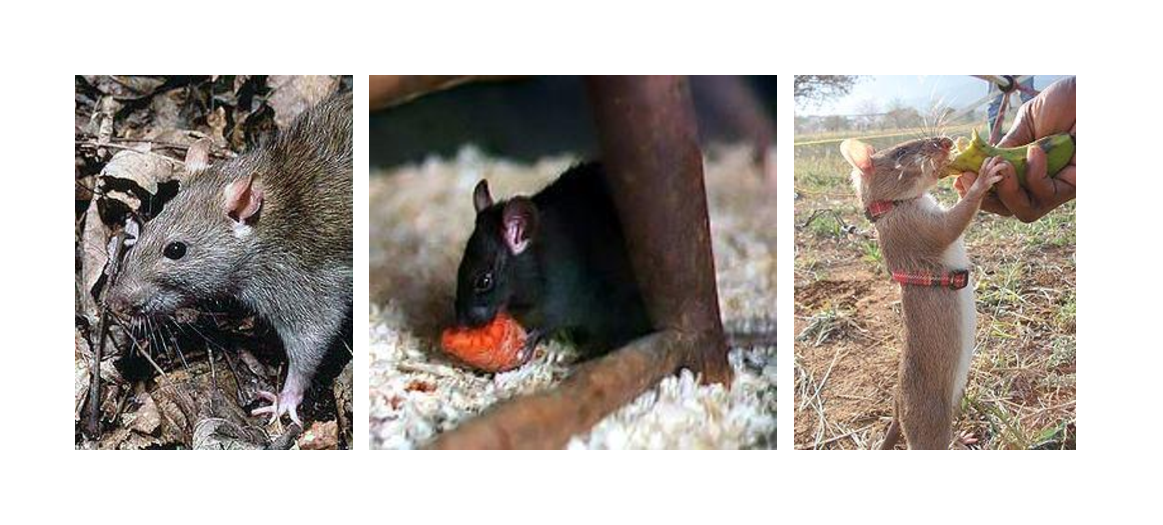
\includegraphics[width=6in,trim={0 .4in 0 .4in},clip]{RatVariations}
\caption{Left: Brown Rat (\textit{Rattus norvegicus})~\cite{BrownRatWikipedia2014}, Center: Black Rat (\textit{Rattus rattus})~\cite{BlackRatWikipedia2014}, and Right: Giant Pouched Rat (\textit{Cricetomys gambianus})~\cite{GiantPouchedRatWikipedia2014}\\
The three species pictured above are those that will be the primary focus of this project. Note that while all three of these animals are referred to as rats, as they all display characteristics associated with the term ``rat,'' only those two belonging to genus \textit{Rattus}, the brown rat and the black rat, are considered true rats.}
\label{RatVariationsFigure}
\end{figure}

How, then, if not by biological connection, are ``rats'' defined? For the purposes of this project, and in common English usage in general, the term ``rat'' is applied to animals, and specifically rodents, which share certain common physical characteristics as observed by the untrained eye. A basic definition of the term ``rat'' then, is a medium-sized rodent with a long, thin, hairless tail~\cite{Hanson2012}. However, in strict reference to this project, a more specific definition of the term ``rat'' may be any animal that is a member of one of the following three species:
\begin{enumerate}
\item Brown Rat (\textit{Rattus norvegicus}) - Also referred to as the common rat, the grey rat, the wharf rat, the Hanoverian rat or the Norway rat~\cite{Barnett1975, Barnett2001}, this species appears on every continent (with the exception of Antarctica), though it originated in Central and Southeast Asia~\cite{ONeill}. All domestic rat strains - ``groups of individuals which share a presumed common ancestry and have clear cut physiological but not usually morphological distinctions''~\cite{Hanson2012} - are members of this species, and of the three species of rat discussed in this text, these share the closest connection to humans in the modern age. While the name is somewhat misleading (the ``brown'' rat is not always brown - tending, in fact, towards white and/or black in domestic strains), this species is referred to as the brown rat throughout this project.
\item Black Rat (\textit{Rattus rattus}) - Also referred to as the old English rat, the blue rat, the roof rat, the alexandrine rat, or the ship rat~\cite{Barnett1975, Barnett2001}, this species is present "throughout Africa, southern Asia, Australia, and the southern coast of the United States", though like the brown rat it is native to Central and Southeast Asia~\cite{ONeill, Zelnio2011}. Until recently, when it was replaced by the brown rat, this species had the greatest impact on humans in Europe~\cite{Barnett2001}. This is the species most closely associated with, and in some sense responsible for, the Black Plague. As with the brown rat, while the name is misleading (the ``black'' rat is, in fact, very rarely black), this species is referred to as the black rat throughout this project.
\item Giant Pouched Rat (\textit{Cricetomys gambianus}) - Also referred to as the African giant pouched rat or the Gambian pouched rat~\cite{APOPO}. As the name implies, this species is large, weighing up to 1.5 kilograms, and have cheek pouches similar to a hamster~\cite{APOPO}. This species is not a true rat, but it does fit within the definition of the term ``rat'' that has been established for this project, and in the English language in general. And while this species does not feature prominently in connection with human history, it does play a interesting role in current rat-human relations, and is therefore included within the context of this project.
\end{enumerate}

Finally, having established the definitions of ``rat'' and ``human,'' I believe it is necessary to clarify what is meant by the term ``co-evolution'' within the contexts of this project. The histories of rats and humans are tightly intertwined. As has already been established, these are two of the most widely successful animals on the planet, with rats following in the wake of human footsteps to almost every corner of the globe (with the exception of the polar regions). And from this relationship, it is possible to discern evidence of co-evolution. This equates to very literal, biological evolution for rats, while with humans it is more abstract - a cultural and technological evolution, of sorts.

Having at this point defined the terms necessary for to understanding this project, it is now possible to discuss the intersections of rats and humans in greater detail.

\section{Biology} \label{Biology}

The first section of this project focuses on the biological aspects of the relationship between rats and humans. This analysis is broken down into two subsections. Subsection~\ref{Taxonomy} provides a comparison of rat and human taxonomy, while Subsection~\ref{Co-Evolution} examines evidence of co-evolution between the two animals.

\subsection{Taxonomy} \label{Taxonomy}

Rats and humans, as it turns out, are remarkably similar creatures at the biological level. To begin an understanding of this, first consider the eight major taxonomic ranks within biological classification, and where rats and humans fit into this system:
\begin{enumerate}
\item Domain - The highest taxonomic rank. Rats and humans are classified within the domain \textit{Eukarya}: our cells consist of a nucleus and other organelles enclosed within a membrane.
\item Kingdom - The second highest taxonomic rank. Rats and humans belong to the kingdom \textit{Animalia}: we are both animals, multicellular organisms with fixed body plans, capable of spontaneous, independent movement. We must also ingest other organisms in order to survive.
\item Phylum - The third highest taxonomic rank. Rats and humans are members of the phylum \textit{Chordata}: we are both vertebrates; we possess a spine and spinal cord.
\item Class - The fourth highest taxonomic rank. Rats and Humans belong to the class \textit{Mammalia}: we are both mammals. We are warmblooded, give birth to live young, nurse young with breast milk, and possess hair.
\item Order - The fifth highest taxonomic rank. At this point, rats and humans have separated. Rats belong to the order \textit{Rodentia}, while humans belong to the order \textit{Primates}. Rats, as rodents, have incisors that will grow continuously throughout the life of the animal. Rodents must gnaw in order to wear these incisors down; if not, their jaws would eventually lock together, either causing the animal to starve or the incisors to pierce the skull. Humans, as primates, have a grasping ability attributable to the possession of opposable thumbs, and possess large brains relative to body size, but are otherwise fairly unspecialized.
\item Family - The sixth highest taxonomic rank. Rats are members of the family \textit{Muridae}, while humans are members of the family \textit{Hominidae}. Rats, as murids, are characterized by their slender bodies, scaled tails, whiskers, and pointed snouts. Rats also demonstrate the strong senses of hearing and smell and frequent breeding habits typical of murids. Humans, as hominids (commonly referred to as the ``Great Apes''), are bipedal and demonstrate an erect posture.
\item Genus - The seventh highest taxonomic rank. Rats are classified within the genus \textit{Rattus}, while humans are classified within the genus \textit{Homo}. Rats (or ``true rats''), as described in Section~\ref{Definitions}, are medium-sized murids with long, thin, hairless tails. Humans, also described in Section~\ref{Definitions}, are the only surviving species of the genus \textit{Homo}.
\item Species - The lowest taxonomic rank. There are many species within the genus \textit{Rattus} (though this project, as discussed in Section~\ref{Definitions}, is primarily concerned with two - the brown rat \textit{Rattus norvegicus} and the black rat \textit{Rattus rattus}), but only one extant species (\textit{Homo sapiens} or \textit{Homo sapiens sapiens}) within the genus \textit{Homo}.
\end{enumerate}
As may be determined from this list, rats and humans split off below the class level into their respective orders, with our unity as mammals divided between rodents and primates. However, there are additional ranks interspersed among these main eight, and upon closer examination we will find that there is a rank between class and order where rats and humans are still linked. This is the clade, or the superorder, and both rats and humans are classsified within the clade \textit{Euarchontoglires}. This rank indicates some of the most exclusive taxonomic characteristics that we both share; primarily, we both have complex jaw muscles in order to control chewing.

Outside of those determined by our mutual taxonomy, rats and humans share many other similarities. We are both omnivores, and consume many of the same foods. We also share the same basic physiology, and have similar organs and body plans~\cite{RatGenomeDatabase, Ensembl2014, Spencer2012}. This similarity has made significant impacts on rat-human relationships, which are discussed in greater detail later on in this project, and in particular in Subsections~\ref{Disease} and~\ref{Research}.

\subsection{Co-Evolution} \label{Co-Evolution}

As mentioned in Section~\ref{Definitions}, as a result of the close contact between rats and humans for much of recorded history, it was inevitable that co-evolution would occur at some point. Again, however, this co-evolution has manifested itself in different ways between the two animals. In technical terms, co-evolution is defined as ``evolution involving successive changes in two or more ecologically interdependent species that affect their interactions''~\cite{CoevolutionDefinition2014}. For rats, this definition of co-evolution may be applied very literally; rats have been biologically altered as a result of their relationship with humans. For humans, however, this definition is perhaps somewhat more abstract. While it could be argued that some biological changes have occurred in humans as a result of human interactions with rats - for example, medical research on rats has significantly increased human knowledge of (and by extent ability to fight) certain diseases - these changes cannot accurately be described as evolution. However, in terms on cultural and technological ``evolution,'' rats have greatly impacted humans. These topics are discussed in later sections of this project. Here, however, the focus is on biology, and therefore predominately concerns itself with the human impact on rats.

The first potential evidence of co-evolution presented here stems from the almost complete disappearance of the bubonic plague from the late seventeenth century onward. One theory as to why this occurred is that some rats developed immunity. Following the principles of evolution, then, ``most of the non-resistant rats may have died leaving only resistant rats''~\cite{ONeill}. And, if the new populations of immune rats were not dying, the fleas that transfered the plague from rat to human had no reason to seek out new (human) hosts~\cite{ONeill}.

If we step backwards in time, we will find that the spread of the plague tended to follow trade routes. This makes sense, because the food that was moved along these routes would have attracted rats, at least some of which would have been infected. The rats would then settle in massive nests in European settlements, attracted by the squalid living conditions in medieval Europe. Under these circumstances, the fleas moved freely from rat to rat, quickly infecting most of the population. When the rats had died, the fleas turned to human hosts. In order to survive among humans, where conditions were for the most part favorable, it was therefore in accordance with the logic of evolution for the rat to develop immunity to the plague~\cite{ONeill}. And, as it so happened (assuming this theory to be true), this development proved to be favorable for humans as well.

The second example is in the extent of human food losses incurred by rats, documented in the following passage:

``Conservative estimates have previously indicated that one fourth of the world’s food supply is damaged annually by rats, and recent evidence from Turkey suggest that rats help consume up to fifteen percent of Turkey’s grain and legume storage. Prosperous and food-rich nations, such as America, suffer high losses because of the rats. In one estimate, food losses incurred due to rats cost almost nineteen billion dollars a year for Americans. In America, the costs are largely monetary, as food supplies are too massive to be consumed in their entirety. On the contrary, small island nations struggling against Malthusian limits face far greater peril when confronted with the bottomless appetite of the rat''~\cite{ONeill}.

The cause of this damage, it may be argued, is co-evolution. Rats have become dependent upon the vast and consistent food supplies readily available through living in close contact with humans. This manifests itself in their continued reliance on human food sources, and in their capacity to decimate biodiversity within fragile ecosystems in situations where they are introduced and then left to their own devices~\cite{ONeill}.

The third and final indication of biological co-evolution discussed within this project may be found in how humans have immortalized the rat in literature, in the wealth of stories and legends that permeate almost every culture across the planet. Much of this literature presents the rat as a creature to be feared and distrusted. While not inherently biological in nature, the consistency in the depiction of rats in these stories may hint at the presence of instinct within the rational human brain. The next section of this project documents the general opinion of rats that may be gathered from the stories of various human cultures. The question left to be answered is if these ideas are taught, or instinctively known.

\section{History} \label{History}

This section provides an outline for some of the histories between rats and humans, arising from various cultures ranging across the planet (Figure~\ref{WorldMapFigure}). However, a few notes in advance. First, this is, of course, by no means an exhaustive list of the cultures in which rats appeared, and even for the limited list of cultures discussed within this section, the information presented is not by any means complete. Second, while some of these histories use the terms ``mouse'' or ``mice,'' in all likelihood they are actually referring to rats, based upon description, and the fact many ancient cultures did not have words to distinguish the two animals. The term ``rat'' itself did not exist in the English language until 1378~\cite{ONeill}.
\begin{figure}
\centering

\includegraphics[width=6in,trim={0 .4in 0 .4in},clip]{WorldMap}
\caption{World Map~\cite{VisitedCountries2014}: Countries Discussed Marked in Red\\
Note: Some of the countries marked are approximations, rather than the exact locations of the cultures discussed. For example, Egypt is marked, because ancient Egypt is discussed. However, the influence of ancient Egypt was geographically larger than modern Egypt. Similarly, South Africa is marked. However, the cultural practices discussed in association with South Africa were likely practiced throughout southern Africa, as opposed to strictly the country of South Africa.}
\label{WorldMapFigure}
\end{figure}

\subsection{Africa} \label{Africa}

In Africa, representations of the rat within human culture largely extend from spiritual or religious belief systems. While rats are considered to be a part of the natural order, their role in the world is predominately negative. However, it is also important to take into consideration that the practices and beliefs regarding rats were not entirely unfounded, and often had a solid basis in maintaining human health and safety.

\subsubsection{Egypt} \label{Egypt}

In ancient Egypt, the rat was a symbol of ``both utter destruction and wise judgment''~\cite{ONeill}. However, the predominant view of rats seems to lean toward the negative, although they were considered a part of the natural order.

Evidence to support the rejection of the rat in Egyptian culture may be found in the great honor and respect assigned to cats. Considered sacred, cats were sometimes mummified, and the killing of a cat was considered a crime punishable by death. An explanation for these practices may be found in the deification if the cat. The feline Mafdet, later known as Bast, was the goddess of protection and execution. These responsibilities represent the importance of the cat in controlling rats - it was the task of cats to `protect' humans and their food stores from rats, and to `execute' rats which dared to invade human space.

\subsubsection{Israel} \label{Israel}

Within the Bible (\textit{Leviticus} 11:1-47), the God of the Israelites provides a lengthy categorization of clean and unclean animals. A significant portion of this text is devoted to rats and related animals:

``Of the animals that move along the ground, these are unclean for you: the weasel, the rat, any kind of great lizard, the gecko, the monitor lizard, the wall lizard, the skink and the chameleon. Of all those that move along the ground, these are unclean for you. Whoever touches them when they are dead will be unclean till evening. When one of them dies and falls on something, that article, whatever its use, will be unclean, whether it is made of wood, cloth, hide or sackcloth. Put it in water; it will be unclean till evening, and then it will be clean. If one of them falls into a clay pot, everything in it will be unclean, and you must break the pot. Any food you are allowed to eat that has come into contact with water from any such pot is unclean, and any liquid that is drunk from such a pot is unclean. Anything that one of their carcasses falls on becomes unclean; an oven or cooking pot must be broken up. They are unclean, and you are to regard them as unclean. A spring, however, or a cistern for collecting water remains clean, but anyone who touches one of these carcasses is unclean. If a carcass falls on any seeds that are to be planted, they remain clean. But if water has been put on the seed and a carcass falls on it, it is unclean for you''~\cite{Bible}.

Of the 47 verses that make up this chapter, it is worth noting that 9 (\textit{Leviticus} 11:29-38) are devoted to specifically to rats and their equals in uncleanliness (quoted previously), and another 7 that may be applied to rats. The second largest count, at 7 verses (\textit{Leviticus} 11:13-19), applies to unclean ``birds'' (quoted next - note that the term ``bird'' refers here not strictly to birds, but to animals capable of flight), but notice that the content between the two is markedly different:

``These are the birds you are to regard as unclean and not eat because they are unclean: the eagle, the vulture, the black vulture, the red kite, and kind of black kite, any kind of raven, the horned owl, the screech owl, the gull, any kind of hawk, the little owl, the cormorant, the great owl, the white owl, the desert owl, the osprey, the stork, and kind of heron, the hoopoe and the bat''~\cite{Bible}.

The section on birds is straightforward: here is a list of the birds that are unclean, do not eat them. The section which refers to rats and their counterparts is far more detailed: here is list of animals that are unclean, do not eat them and do not touch their carcasses; if you do, or if their carcasses come into contact with any of possessions, here are the correct cleansing procedures. The threat level for rats is much higher.

It is often stated that the reasoning behind the categorization of animals into clean and unclean categories largely related to health concerns, and in particular dietary concerns. This however, does not explain the added emphasis for rats. A possible explanation, however, may be found on the level of contact. The birds listed above were mostly likely not a part of the daily lives of humans. Therefore, it was sufficient to simply say ``these are unclean, do not eat them,'' and leave the issue at that. Rats, on the other hand, probably were a constant presence. In this case, it would make sense that additional precautions be attached.

\subsubsection{South Africa} \label{South Africa}

In South Africa, views on rats continued to extend from a largely spiritual or religious tradition. Warriors twisted tufts of rat hair into their own, giving them the agility of the rat that would help them to avoid death~\cite{Barnett2001}. Unlike the traditions of Egypt and Israel, however, this representation is far more neutral, and even positive, in the sense that a neutral rat ability (agility) is used for the protection of human life.

\subsection{Asia} \label{Asia}

The black rat and the brown rat, the two species most closely intertwined with humans throughout history, are believed to have their origins in Asia. As such, it is from these cultures that some of the most ancient accounts of rat-human relations arise. While the rat here, as elsewhere, is still viewed as a threat, particularly in relation to food sources, the reputation of the animal overall fares better here, where the rat is often representative of an intelligent, stylish, and even charming personality.

\subsubsection{China} \label{China}

In China, the rat is the first of the animals that appears in the twelve year Zodiac cycle. As with every animal in this cycle, the rat has a set of both positive and negative traits associated with it. Those born during the ``Year of the Rat'' are considered to possess the positive traits of ambition, intelligence, charm, artistry, and eloquence. However, they also carry negative traits that fit into an almost universal opinion of rats: vindictiveness, manipulativeness, selfishness, self-destructiveness, arrogance, amorality, and greed~\cite{Barnett2001}.

\subsubsection{Japan} \label{Japan}

In Japan, the rat is again imbued with positive qualities, the foremost of which is good fortune. The rat is a messenger of wealth, and it is said that if the rats eat the first rice cakes of the New Year, the harvest will be bountiful~\cite{Marrin2006}.

Rats also had tangible worth. In ancient Japan, the whiskers of rats were sought by artists for their brushes, which made possible the delicate details found in traditional painting~\cite{Barnett2001}.

\subsubsection{India} \label{India}

India is widely accepted to be the birthplace of both the black rat and the brown rat, and as such, it makes a certain amount of sense that possibly the oldest account of rats appears here. In the \textit{Atharva Veda}, a sacred Hindu text dating back to the second millennium BCE (possibly as early as the late third millennium BCE), there is curse against rats: ``O, Ashwini. Kill the burrowing rodents which devastate our food grains, slice their hearts, break their necks, plug their mouths, so that they cannot destroy our food''~\cite{Barnett2001}.

Despite this threat of violence, the rat makes an unexpected appearance at the feet of a Hindu deity. Ganesha, four-armed with the head of an elephant, is the god of literacy and learning. He is closely associated with rats~\cite{Barnett2001}. The significance of this is debated. One explanation is tied to the representation presented in the \textit{Atharva Veda}, with rat as destroyer. In this depiction, the rat is subservient to Ganesha, the destroyer conquered by the overcomer. An alternative viewpoint claims that the rat is a symbol, indicating that Ganesha is capable of appearing in even the most secret of places.

However, the rat is not viewed in a negative light everywhere in India. Rats carry positive connotations for the Karni Mata cult of a Jain temple in Deshnoke, Rajastan. Here, rats are worshiped as ancestors~\cite{Edelman2005}.

\subsection{Europe} \label{Europe}

Europe, it appears, is not a particularly good place to be a rat. The vast majority of representations of the rat in European culture depict it as a vile, evil, filthy, murderous creature. At the same time, however, it is interesting to note that the rat appears to be far more marketable in many European histories than in the others that have been discussed in this project. The same humans who condemned the rat, it seems, had no qualms in turning it in for a profit.

\subsubsection{England} \label{England}

In England, rats were viewed as killers. The following passage from the George Orwell novel \textit{Nineteen Eighty-Four} is just one example of the fear that the rat inspired: ``a woman dare not leave her baby alone... even for five minutes. The rats are certain to attack it. Within quite a small time they will strip it to the bones''~\cite{Barnett2001}. But while there are various accounts of rats attacking and even killing humans, this is far from the norm. While perfectly well adapted to live alongside human activity, wild rats, like many other animals, have learned to fear humans. In principal, a wild rat will not approach a human.

However, as with many of the cultures previously mentioned, rats were also recognized as having positive qualities. One account describes the compassion of rats for their own kind:

``Although its disposition appears to be naturally exceedingly ferocious... an anecdote [of a rat] exhibiting a degree of tenderness and care towards the disabled and aged members of their community... an old blind Rat, which held a piece of stick at one end in its mouth, while another Rat had hold of the other end of it, and thus conducted his blind companion''~\cite{Barnett2001, Marrin2006}.

And, of course, regardless of whether the rat was a creature of good or evil, it was never a crime to use it for profit. During the fourteenth century, rat skins were sold for one farthing apiece~\cite{Barnett2001}. While the monetary value of a farthing only amounted to a quarter or a penny, this was, at the time, considered a useful amount. Later, in the 1800s, and possibly as early as the late 1700s, the popularity of ``rat baiting'' - a pub sport which consisted of emptying dozens of rats from sacks into pits, setting dogs on them, and spectators placing bets on how many rats the dogs could kill - provided plentiful income to ``rat catchers'' (these topics, and their impact on the domestication of the rat are discussed in further detail in Subsection~\ref{Companionship}).

\subsubsection{France} \label{France}

In France, we find an eerie echo of the \textit{Atharva Veda} discussed in Subsubsection~\ref{India}, wherein the Bishop of Autun put rats under a formal curse~\cite{Barnett2001}.

This fear of rats, however, does not seem to have prevented the French from eating them as delicacies. First published in 1938, the \textit{Larousse Gastronomique} provides directions on how to properly prepare rat flesh for gourmet consumption: skin and clean, then season with oil and shallots and grill over an open fire~\cite{Barnett2001}.

\subsubsection{Germany} \label{Germany}

One of the more unique stories found in researching this project comes from Germany. Here, there existed a practice of throwing the temporary tooth of a child backward over one's head, accompanied by an incantation requesting rats to provide the child with an `iron' tooth~\cite{Barnett2001}. This practice likely is the predecessor to the American ``tooth fairy.''

\subsubsection{Greece} \label{Greece}

Another interesting occurrence appears in Greek culture. Unlike many European cultures, where the rat is viewed also exclusively as a creature of danger, the Greeks seem to have a more balanced view. In Ancient Greece, for example, and its surrounding cultures, ``mice'' were revered as ``both the protectors and destroyers of crop''~\cite{ONeill}.

Moreover, this idea does not seemed to have fallen with classical Greece. More recently, we find a similar example, in which it is claimed a farmer wrote the following note to the rats attacking his crops: ``I adjure you, ye mice here present, that ye neither injure me, nor suffer another mouse to do so. I give you yonder field. But if I catch you here again, by the mother of the gods, I will rend you in seven pieces''~\cite{Barnett2001}.

\subsection{North America} \label{North America}

This subsection, unlike the previous few, is not broken down into multiple subsubsections by country, on the basis that only one country is discussed - the United States. Here, we find human attitudes toward rats to be remarkably similar to those in Europe, and in particular England. Considering the United Sates started off as colony of England, this makes a certain amount of sense. A note on the content of this subsection: the English, obviously, were not the first in North America. Native Americans had already lived here for thousands of years. The content of this section does not discuss Native American attitudes towards rats. It should be recognized, however, that when the brown rat was introduced to North America by Europeans, this animal had a significant impact on the local ecosystems, and by extent the human populations that depended on those ecosystems for survival. While this is not discussed here, it also should not be ignored.

When Europeans came to the United States, the rats followed. And with these rats came the European fear and disgust so closely associated with them. In the Edgar Allan Poe story \textit{The Pit and the Pendulum}, we find a passage that echoes the tone and emotion of \textit{Nineteen Eighty-Four}:

``They pressed - they swarmed upon me in ever accumulating heaps. They writhed upon my throat; their cold lips sought my own; I was stifled by their thronging pressure; disgust, for which the world has no name swelled my bosom and chilled, with a heavy clamminess, my heart''~\cite{ONeill}.

The fear is evident in this passage; interestingly enough, however, it is through the work of the rats that our protagonist eventually narrowly escapes death.

And, as in England, we can occasionally find an undercurrent of human sympathy and compassion of the hated rat. For example, it is claimed that farmer once wrote a letter to his rats explaining that crops were short and that he could not afford to keep the rats during the winter, requesting that they take his neighbors' grain instead~\cite{Barnett2001}.

This, then, is a very general overview of the histories of rats and humans. The final goal of this project is to extend the influence of this relationship into the present. In the last few centuries, significant new facets have appeared in the connection between rats and humans, and while in many ways these changes have brought enlightenment and understanding, they have also created potential concerns. This it the task of Section~\ref{Connections}.

\section{Connections} \label{Connections}

In Section~\ref{History}, this project covered a handful of the historical dynamics of rat-human relationships across the planet. This section, in a sense, is merely a continuation of the previous. However, it has been separated, for two reasons.

First, there is the growing phenomenon of globalization. While historically, there were connections between cultures, through trade and other means, and these cultures did influence each other, a few examples of which are discussed above, for the most part, various cultures were distinct and separate from one another. Today, however, this is becoming less and less the case, with such innovations as faster modes of transportation, and instant communication networks like the internet. The aspects of the rat-human relationship discussed in this section are more recent, and therefore, are far more global in nature than connected to any specific locality.

Second, the cultures in the previous section were, for the most part, simply presented. While there was some discussion of why these histories came to exist, this analysis was fairly limited. In this section, however, the developments presented are considered much more thoroughly.

In \textit{Rats are people, too!: Rat-Human Relations Re-Rated}, Birgitta Edelman argues that the modern rat has a ``triple identity'': the positive of rats as pets, the negative of rats as vermin, and the neutral of rats as laboratory animals~\cite{Edelman2002}. In this project, this break down is generally accepted, and these three categories are indeed presented and discussed. However, this project also considers a fourth category: the rat as service animal. This has been done because the role of service animal does not neatly fit into any of the other categories: the service animal is certainly not a vermin, but neither is it quite a pet, and it does not serve the same function as a laboratory animal. On the scale from positive to neutral to negative, pet to laboratory animal to vermin, the service animal is probably best described as a positive-neutral, somewhere between the pet and the laboratory animal.

\subsection{Disease} \label{Disease}

First, there is the rat as vermin. Perhaps the most obvious reason for this categorization is the association in the human mind of rats with disease.

For instance, rats are often blamed as the source of one of the ``deadliest epidemiological disasters of human history''~\cite{ONeill}. This disease was the bubonic plague, commonly known as the Black Death, which spread across Europe from 1347 to 1351, killing one in every three people~\cite{Gottfried1983}. And to an extent, it is true; the disease originated in the rodent populations. But rats were not immune; on the contrary, they were the first to die. When the rat population had depleted, only then did the fleas that transfered the disease from rat to human seek out human hosts~\cite{Marrin2006, ONeill}. The point being, while they certainly had their role to play, it is unfair and untrue to place all the blame on the shoulders of rats.

However, there is another reason behind the view of rat as vermin, in this case far more abstract. The brown rat is believed to have arrived in England in 1728, and to have completed its spread across the country by 1800 (note that the brown rat here displaces the previously well established black rat)~\cite{Edelman2002}. During the early 1800s, it is argued, the image of the rat went through a transformation, from ``despised'' to ``disgusting''. Previously, the rat had merely been a nuisance: invading houses and barns, and eating and soiling food intended for human consumption. With the development of the sewer system, however, the rat became synonymous with dirt and refuse, thereby making it abhorrent. The sewer became a physical underworld, intended to hide filth from sight and smell. The rats, which happily and readily entered into this underworld, were similarly rejected~\cite{Edelman2005}.

Interestingly enough, it is during this same period, when the rat is being transformed from a ``despised'' animal to a ``disgusting'' animal, that the two other primary identities of the rat, as laboratory animal and as pet, came into existence. These simultaneous occurrences are explored in the following two subsections.

\subsection{Research} \label{Research}

Second, there is the rat as laboratory animal. The first documented experimentation on rats dates back to 1856 in France, followed closely over the next few decades by experiments in England, Germany, and the United States~\cite{Edelman2002}. It is interesting, however, to note that experiments were occurring alongside the transformation of the rat from ``despised'' to ``disgusting,'' a process covered in the previous subsection.

How is this? One possible explanation is that the rat was chosen for experimentation simply because of its lowly status. In England, human dissection was prohibited until the 1500s, and was still largely limited and taboo until the first half of the 1800s. However, the human was, according to the England, separate from the animal: the human had a soul. Therefore, rats, as soulless animals, and low status animals at that, were free game.

Another explanation is the physical and economic advantages of the rat. Rats were small, easy to hand and reproduce, fairly low maintenance, quick to mature, and had short lifespans~\cite{Edelman2002}. These qualities well suited the rat to use in experiments and the laboratory environment.

Whatever the reason, the choice of rat as laboratory animal turned out to be a wise one. As discussed in Subsection~\ref{Taxonomy}, the rat and the human share a remarkable number of physical similarities. We share similar organs, body plans, even dietary habits and aging processes. And, as a result, we are susceptible to many of the same diseases and other issues, which makes the rat an excellent research subject in an attempt to better understand and help humans and human bodies.

For example, by implanting cancer cells in rat bodies, we are better able to understand how cancer roots and spreads in human bodies. By exposing rats to tobacco smoke, a correlation was made between tobacco smoke and lung cancer. By testing anti-rejection drugs on rats, researchers have been able to save the lives of many surgical patients. Similarly, by testing vaccines on rats for treatment of certain diseases, researchers are better able to understand how the drugs with effect humans, to know whether they with help or hurt~\cite{Marrin2006}.

Many scientific and medical advances have been made through research using rats, only a handful of which have been listed here. It is not in the interests of this project to negate these discoveries. But animal testing is also a controversial issue, for reasons which are worth discussing here.

Objections to animal experimentation often stem from the idea of ``speciesism'' - ``prejudice or attitude or bias in favor of the members of one's own species and against those of members of other species''~\cite{Phoenix2005}. This is the definition given in the 2005 film \textit{Earthlings}, where the concept is compared to prejudices including racism and sexism. However, if these phenomena are in fact comparable, the definition provided is incomplete. In the cases of racism and sexism, while prejudice is certainly a necessary element, there must also be the power to institutionally enforce that prejudice. The dynamics of these systems ensure that certain privileged individuals benefit from this institutionalized prejudice - whether they wish to or not, whether they approve of the system or not.

With this in mind, let us return to the concept of speciesism. The first ingredient, prejudice, is obviously present. Humans have long considered themselves superior to ``the Beast.'' The second is also readily apparent. One need only look at the meat industry, fur fashions, and - indeed - animal testing facilities. In these instances, humans have everything to gain, and animals (or, in the interest of accuracy, non-human animals - we are all, human or otherwise, animals) pay the price.

Those who object to idea of speciesism often bring up the concept of ``anthropomorphism.'' Anthropomorphism is strictly defined as ``attributing human characteristics to things not human,'' but in practice translates to ``attributing characteristics that belong only to humans to things not human''~\cite{Milton2005}. And herein lies the issue with anthropomorphism. Humans, again, like to believe themselves superior to all other animals. But there is more and more research being produced every year that indicates that this is not necessarily true. For example, in the last three years, there has been research conducted which indicates that rats feel regret and learn from poor decisions in a similar manner to humans~\cite{Lewis2013, Lewis2014} and even feel empathy and compassion~\cite{Brown2011}. The point being, it is unfair to cry anthropomorphism, to claim that an animal exhibits a human trait, when that trait clearly belongs to the animal as well.

These ideas are pushed further by the third main identity of the rat as pet. This is the topic of the next subsection.

\subsection{Companionship} \label{Companionship}

Third, there is the rat as pet. And, as with the appearance of the laboratory rat, we find this identity beginning to form at approximately the same time the rat was being redefined from ``despised'' to ``disgusting.''

As briefly mentioned in Subsubsection~\ref{England}, during the middle of the 1800s, the sport of ``rat baiting'' became rather fashionable. While the practice was fairly short lived, it did provide ``rat catchers'' with an extra source of profit, in addition to their traditional role as exterminators. However, particularly innovative rat catchers discovered yet another means of making a profit off their chosen profession.

Some rat catchers, including ``Her Majesty's Rat Catcher'' Jack Black, discovered that they could breed rats for color and temperament, and sell these specimens, primarily to upper class women, for a relatively high price. To the rat catchers, the rat was solely a source of income; there was no sentimental value attached to them, no concept of them as living, feeling beings. But for the women who chose to purchase them, they were pats, companions, and even friends~\cite{Edelman2002, Edelman2005}. As a self-identified ``crazy rat lady'' writes:

``They [the rats] are very playful, playing the attack rat, jumping, popping up in the air, playing Boo with me, pretending to run away, only to quickly turn back thinking they fooled me. I love their wet cold noses. They are alive and can think, comfort you when sad, make you laugh, lave little hands with fingers to reach out to you. They make me feel loved and when all is calm and quiet and they're in my lap and I can feel their warm breath on my skin, I cannot express the feelings I get''~\cite{Edelman2005}.

But how did this attitude come to exist? The perspective of the rat catchers fits within the idea of the rat as ``disgusting.'' This is not so for the rich women who kept these animals as pets. However, as with the previous identities of the rat discussed within this project, there are multiple possible explanations.

The first explanation is as simple as separation. These women had little to no contact with the ``disgusting'' sewer rat, and therefore, to their eyes, the rat could simply exist as yet another animal, even a lovable, adorable, and charming one.

A second explanation is also based in separation, but at a different level. In this scenario, the woman recognizes her pet rat as belonging to the same species as the ``disgusting'' rat, but to her, the individual triumphs over the group. As an example, the lower classes were often categorized in a similar manner to the rats: this was a group to be looked down upon, and viewed with disgust. However, just because the group was ``disgusting'' did not bar the individual from redemption. In this respect, the rats were to the women as Eliza is to Professor Higgins in \textit{Pygmalion}, a charming ``oddity'' of sorts~\cite{Edelman2002, Edelman2005}.

A third explanation is yet again based in separation, albeit again of a different variety. Here, the pet rat is still very much a member of its breed; at its core, it is still the ``disgusting'' sewer rat. But it is also only a single rat, separate from the horde. On it own, the positive qualities of the individual rat are now visible~\cite{Edelman2005}.

The fourth and final explanation presented in this project stands apart from its predecessors, in that its basis is not in separation, but in connection. Here, the pet rat is still very much a low, filthy, and even masculine creature. In keeping the rat, then, these women aimed to establish an identity, even status, for themselves, separate from that assigned them by their gender and class~\cite{Edelman2005}.

In support of this fourth explanation, and as a final note, in recent years, the rat has also achieved some popularity as a status symbol. Individuals identifying within certain subcultures, such as punks or goths, may opt to keep rats as pets precisely because of their association with the low, the filthy, and the frightening~\cite{Edelman2005}.

Here, then, are the three primary identities of the rat: the negative vermin, the neutral laboratory animal, and the positive pet. However, as mentioned at the beginning of this section, this project argues for the inclusion of a fourth identity: the rat as service animal. The next subsection will lay out the foundations for this category.

\subsection{Service} \label{Service}

This project has already covering the three accepted identiteies of the rat, in its roles as vermin, laboratory animal, and pet. However, there is a fourth role that has emerged in recent years, and this is the categorization of the rat as service animal. This category is described here.

One example of this phenomenon is the HeroRATS trained by the organization APOPO (Anti-Persoonsmijnen Ontmijnende Product Ontwikkeling - translated to English as Anti-Personnel Landmines Detection Product Development). APOPO trains giant pouched rats - note that this species is an example of a case where the term ``rat'' is not applied to a true rat, but rather a rodent that demonstrates characteristics humans associate with the term ``rat'' (see Section~\ref{Definitions}) - to detect land mines and, in more recent work, tuberculosis~\cite{APOPO}.

But - Why rats? APOPO lists the following reasons:
\begin{enumerate}
\item Exceptional Sense of Smell - Rats may have up to 1000 different types of olfactory receptors, each coded for by a separate gene. This information alone takes up approximately 1\% of the total genetic code~\cite{Hanson2012}.
\item Intelligent and Trainable - APOPO also mentions, in relation to this information, that the giant pouched rat may have a lifespan of up to eight years, meaning that the rats live long enough to be productive. This point is particularly interesting, and is discussed in detail later.
\item Too Light to Set Off Mines - Giant pouched rats typically weigh about one kilogram, while anti-personnel landmines usually require a weight of about five kilograms to detonate. According to APOPO, a rat has never been injured or killed in the minefield.
\item Locally Sourced and Widely Available - APOPO currently has anti-personnel landmine detection and removal programmes in Tanzania, Mozambique, Thailand, Angola, Cambodia, Vietnam, and Lao PDR; and tuberculosis detection programmes in Morogoro, Tanzania; Dar es Salaam; Tanzania and Maputo, Mozambique. Giant pouched rats are native to three of these countries (and all three cities), and therefore adapted to function within the environment.
\item Easily Transferable Between Trainers - Rats do not tend to bond with particular humans, and so it is easy to move them to various locations as necessary.
\item Low Maintenance Cost - Rats are cheap feed, train, transport, and breed.
\item Resistant Species - As an extension of item 5, as giant pouched rats are native to Sub-Saharan Africa, they are resistant to many potentially detrimental environmental factors.
\end{enumerate}

Here, we see a foundation very similar to that established for the category of the rat as laboratory animal. The explanation is primarily neutral and objective. But it is still not the laboratory animal. For the laboratory animal it has already been established, is readily sacrificed for the benefit of humans. The service animal, however, despite its purpose of benefiting humans, is largely protected from harm. APOPO dedicates a whole section of its Frequently Asked Questions page to ``Animal Welfare,'' and here, in response to the question ``Do animals sometimes get hurt or killed during the mine action job?,'' APOPO provides the following response:

``Demining is a dangerous job and, sadly, human deminers are sometimes injured or killed. The rats have a significant advantage over their human demining partners in that a pressure-activated antipersonnel land mine typically requires about five kilograms of pressure to be activated. Our heaviest operational male rats do not exceed 1.5 kilograms and are, therefore, in no danger of activating this type of land mine. However, working around land mines is dangerous work for anyone involved. Fortunately, no rats have been injured or killed in the minefield to date''~\cite{APOPO}.

Clearly, then, the service animal is not to be harmed. This indicates that the service animal has a ranking somewhere above the laboratory animal, in that it is assigned the right to its own existence. However, the lack of sentimentality in the original explanation for choosing the rat in the first place is a reminder that this animal is certainly not to be mistaken for the pet. The rat as service animal, therefore, lies somewhere in between the positive and the neutral, the pet and the laboratory animal.

\section{Conclusions} \label{Conclusions}

Rats and humans share an extensive and complex history. The purpose of this project was to examine this history, and to attempt to understand the ways in which it has affected the two animals, particularly in a co-evolutionary sense.

In attempting to complete this goal, this project has documented the biological influence of rats and humans on on another, the histories of these two animals throughout a number of world cultures, and the contemporary development of the various identities of the rat.

In conclusion, it is reasonable to argue that, while the human has quite literally affected the evolution and development of the rat, the rat has had a much more subtle, if still very much present, influence on the human. That is to say, from a co-evolutionary standpoint, the human has changed the biology of the rat, while the rat has changed the culture and technology of the human.

\section{Acknowledgments}

Thanks to Leslie Meek for acting as faculty advisor for this project, to Rebecca Dean and Heather Waye for acting as faculty panel members, and to all three for providing indispensable resources and advice.

\pagebreak

\bibliographystyle{acm}
\bibliography{StoryOfRatsBibliographyVersion1}

\end{document}